\section{Общая характеристика состояния атмосферы}
\begin{frame}{\insertsectionhead}
    \begin{columns}
        \begin{column}{.55\linewidth}
        \footnotesize
        Выбросы загрязняющих веществ от стационарных и 
        передвижных источников на территории Саратовской области в 2018 году составили 377,2 тыс. т.
        По сравнению с предыдущим годом выбросы от стационарных источников уменьшились на 4,6 тыс. т (на 3,8\%), а 
        выбросы от автотранспорта увеличились на 10,4 тыс. т (на 4,2\%).
        
        ~ % Invisible

        На протяжении последних лет основными вкладчиками в промышленные выбросы области являются предприятия транспортировки и хранения и предприятия обрабатывающего производства. 
        \end{column}

        \begin{column}{.42\linewidth}
            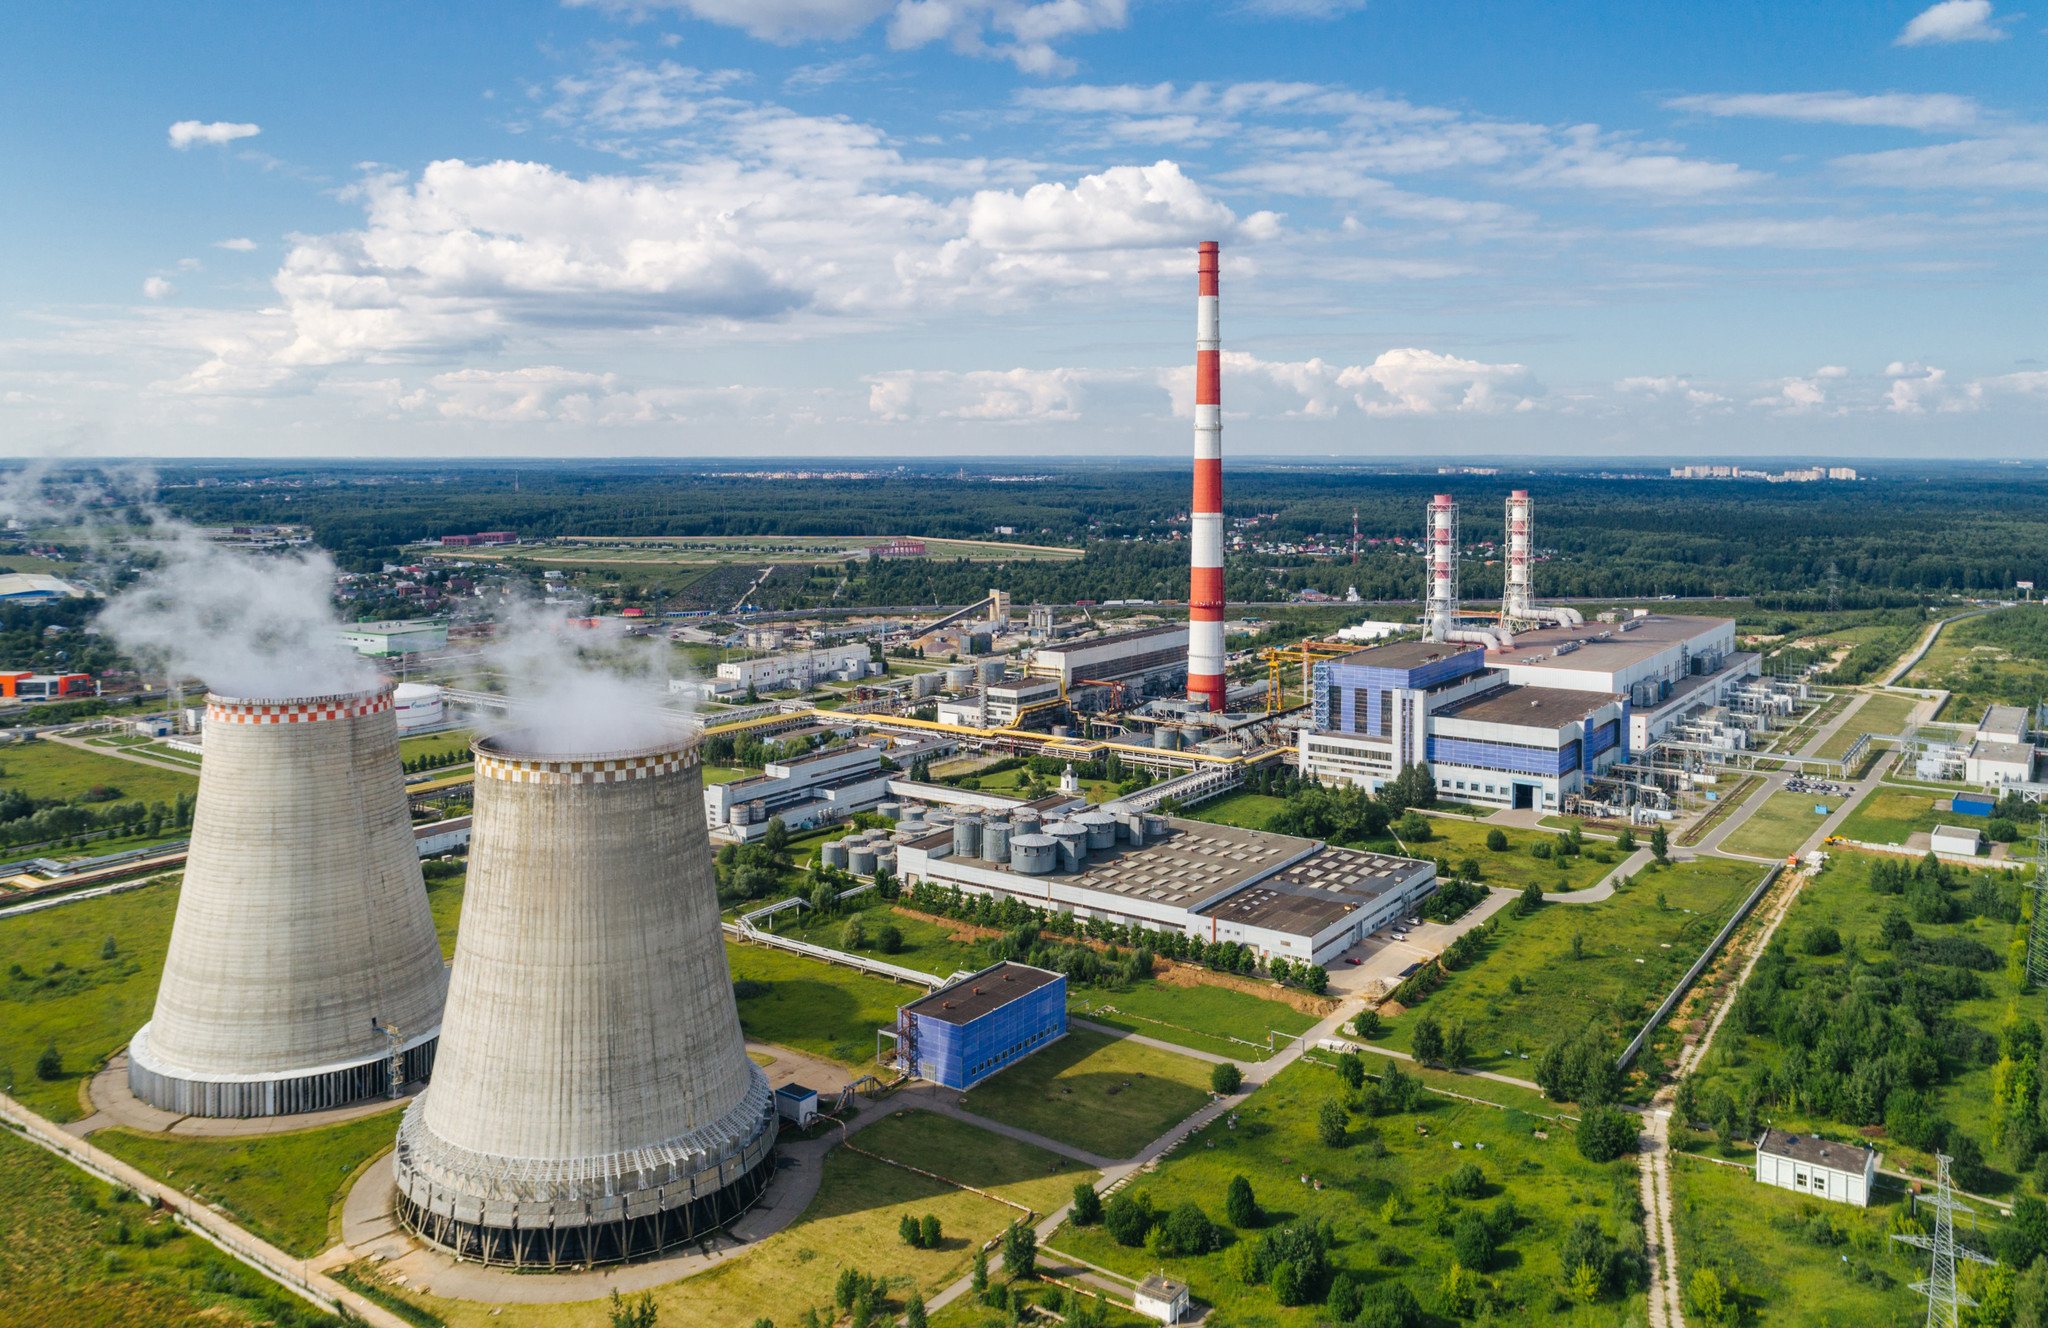
\includegraphics[width=1.1\textwidth]{assets/tes.jpg}
        \end{column}
    \end{columns}
\end{frame}

\begin{frame}{\insertsectionhead}
    \begin{columns}
        \begin{column}{.55\linewidth}
        \footnotesize
        Увеличение выбросов загрязняющих веществ в атмосферу от 
        автотранспорта произошло во всех крупных городах области, что связано с увеличением количества зарегистрированных автотранспортных средств.
        
        ~ % Invisible

        Наибольшее загрязнение атмосферного воздуха регистрируется на улицах с 
        интенсивным движением в точках измерений крупных
        городов области: Саратов, Балаково, Балашов.
        \end{column}

        \begin{column}{.42\linewidth}
            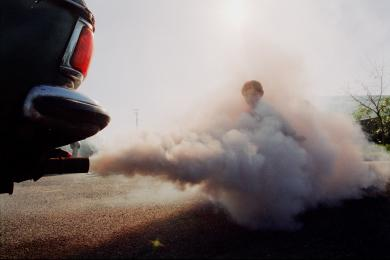
\includegraphics[width=1.1\textwidth]{assets/vihlopi.jpg}
        \end{column}
    \end{columns}
\end{frame}
